\documentclass[12pt]{article}
\usepackage{amsmath}
\usepackage{amssymb}
\usepackage[unicode=true, colorlinks=true, linkcolor=blue, urlcolor=cyan]{hyperref}
\usepackage{graphicx}
\usepackage{float}
\usepackage{caption}
\usepackage{listings}
\usepackage{xcolor}
\usepackage{pgfplots}
\usepackage{tikz}
\usepackage{rotating}
\usepackage{pdflscape}   % Landscape pages
\usepackage{ragged2e} % For justification
\usepackage[a4paper, margin=1in]{geometry}
\usepackage[backend=biber,style=alphabetic]{biblatex} % Bibliography management
\usepackage{booktabs} % For better tables
\usepackage{siunitx} % For SI units
\usetikzlibrary{snakes}
\usetikzlibrary{arrows.meta, shapes}
\addbibresource{references.bib} % Bibliography file
\graphicspath{{tex/}}

% Define colors
\colorlet{punct}{red!60!black}
\definecolor{background}{RGB}{240, 248, 255} % Pale Blue
\definecolor{delim}{RGB}{20,105,176}
\colorlet{numb}{magenta!60!black}

% Define JSON language
\lstdefinelanguage{json}{
  basicstyle=\ttfamily\footnotesize\color{black},
  basicstyle=\ttfamily\footnotesize\color{black},
  numbers=left,
  numberstyle=\scriptsize,
  stepnumber=1,
  numbersep=8pt,
  showstringspaces=false,
  breaklines=true,
  frame=lines,
  backgroundcolor=\color{background},
  literate=
  *{0}{{{\color{numb}0}}}{1}
  {1}{{{\color{numb}1}}}{1}
  {2}{{{\color{numb}2}}}{1}
  {3}{{{\color{numb}3}}}{1}
  {4}{{{\color{numb}4}}}{1}
  {5}{{{\color{numb}5}}}{1}
  {6}{{{\color{numb}6}}}{1}
  {7}{{{\color{numb}7}}}{1}
  {8}{{{\color{numb}8}}}{1}
  {9}{{{\color{numb}9}}}{1}
  {:}{{{\color{punct}{:}}}}{1}
  {,}{{{\color{punct}{,}}}}{1}
  {\{}{{{\color{delim}{\{}}}}{1}
  {\}}{{{\color{delim}{\}}}}}{1}
  {[}{{{\color{delim}{[}}}}{1}
  {]}{{{\color{delim}{]}}}}{1},
}

\setlength{\parskip}{1em}

\lstset{frame=single, showstringspaces=false, columns=fixed, basicstyle={\ttfamily}, commentstyle={\it}, numbers=left, tabsize=4}

\definecolor{codebackground}{RGB}{240, 248, 255}
\definecolor{codecomment}{RGB}{106,153,85}
\definecolor{codekeyword}{RGB}{30,30,255}
\definecolor{codestring}{RGB}{163,21,21}
\definecolor{codenumber}{RGB}{100,100,100}

\lstdefinestyle{modernstyle}{
  backgroundcolor=\color{codebackground},
  commentstyle=\color{codecomment},
  keywordstyle=\color{codekeyword},
  numberstyle=\tiny\color{codenumber},
  stringstyle=\color{codestring},
  basicstyle=\ttfamily\footnotesize\color{black},
  breakatwhitespace=false,
  breaklines=true,
  captionpos=b,
  keepspaces=true,
  numbers=left,
  numbersep=5pt,
  showspaces=false,
  showstringspaces=false,
  showtabs=false,
  tabsize=4
}

\lstset{style=modernstyle}

\begin{document}

\begin{titlepage}
  \centering
  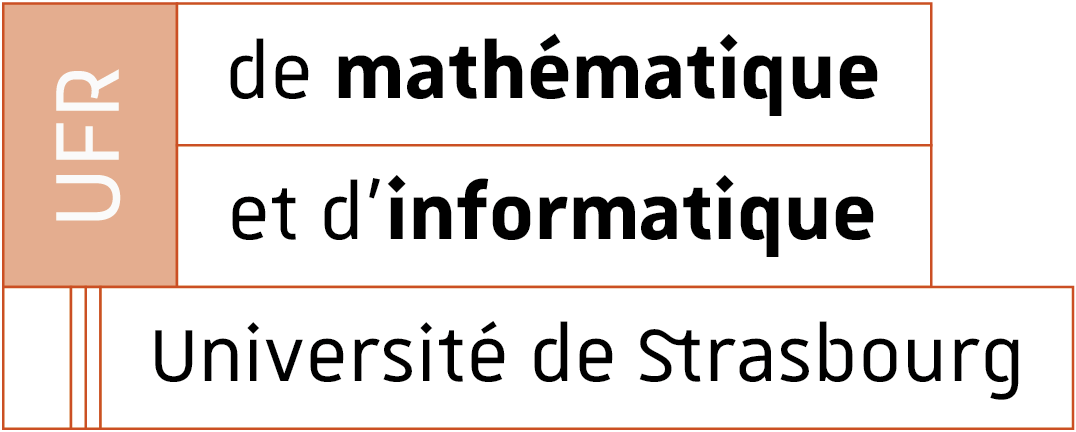
\includegraphics[width=0.5\textwidth]{images/logo-ufr.png}\par\vspace{1cm}
  \vspace{1.5cm}
  {\huge\bfseries M2-Project: \\
  Pre and Post-Processing applied to a LNCMI Bitter Magnet\par}
  \vspace{2cm}
  {\Large Pierre-Antoine Senger and Antoine Regardin\par}
  \vfill

  \vfill

  % Bottom of the page
  {\large Date: \today\par}
\end{titlepage}

\tableofcontents

\newpage

\section{Introduction}

\subsection{Context}
A Bitter magnet is a type of electromagnet that uses stacked, flat, spiral-shaped
copper or brass plates (discs) with slits to allow cooling water to flow through.
Due to their ability to handle large electric currents without overheating and
generating strong magnetic fields, Bitter electromagnets are widely used in
high-field physics research, such as nuclear magnetic resonance (NMR) and magnetic
resonance imaging (MRI) machines.

Simulations of how current and heat are distributed in the magnet are crucial to
understand the behavior of the magnet to maximize its performance and prevent
overheating and irreversible damages.

\begin{figure}[H]
  \centering
  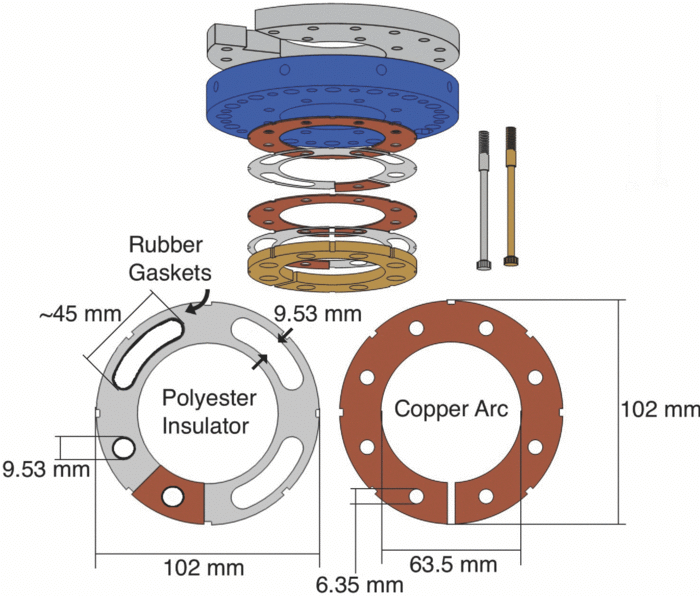
\includegraphics[width=0.8\textwidth]{images/Bitter-electromagnet-breakout.png}
  \caption{Breakout of a Bitter electromagnet \cite{bitter_breakout}}
\end{figure}

\subsection{Main objectives}

\begin{itemize}
  \item Model the Bitter magnet geometry and mesh it with an adaptive mesh.
  \item Run the steady case simulation to study the distribution of current and heat in the magnet.
  \item Visualize the results and analyze the behavior of the magnet.
\end{itemize}

\subsection{Software and libraries}
To make the model of the Bitter and mesh it, we will use Gmsh \cite{geuzaine_gmsh_2009}, a three-dimensional
finite element mesh generator with a built-in CAD engine and post-processor.
Gmsh is an open-source software and is widely used in the scientific
community.

As for our simulations, our primary tool will be Feel++ \cite{christophe_prudhomme_feelppfeelpp_2024}, a robust and
efficient open-source C++ library designed for solving partial differential equations using
the finite element method \cite{fem}.

\section{Methodology}
\subsection{Geometry and mesh generation}

Table~\ref{tab:bitter_geometry} and Figure~\ref{fig:bitter_geometry} describe the
geometry of the LNCMI Bitter magnet.

\begin{figure}[H]
  \centering
  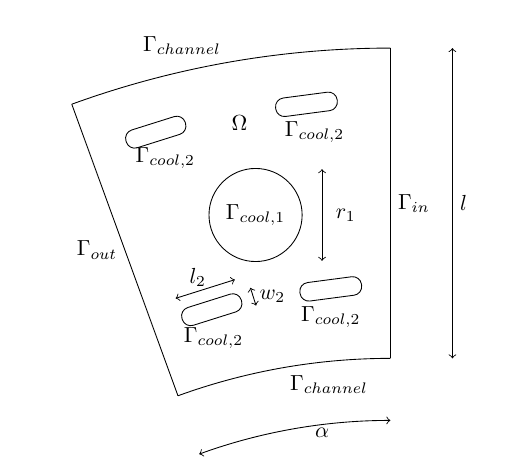
\includegraphics[width=0.8\textwidth]{images/top_view_bitter.png}
  \caption{Top view of the geometry of the LNCMI Bitter magnet.}
  \label{fig:bitter_geometry}
\end{figure}

\begin{table}[H]
  \centering
  \begin{tabular}{p{5cm}p{2cm}p{2cm}p{2cm}}
    \toprule
    \renewcommand{\arraystretch}{1.5} % Adjust row spacing for aesthetics
    \textbf{Parameter} & \textbf{Symbol} & \textbf{Units} & \textbf{Value} \\
    \midrule
    Internal radius & $r_i$ & \SI{}{mm} & 200 \\
    Length of the bitter & $l$ & \SI{}{mm} & 100 \\
    Angle between $\Gamma_\text{in}$ and $\Gamma_\text{out}$ & $\alpha$ & \SI{}{\radian} & $\pi/18$ \\
    Diameter of $\Gamma_\text{cool,1}$ & $r_1$ & \SI{}{mm} & 10 \\
    Width of $\Gamma_\text{cool,2}$ & $w_2$ & \SI{}{mm} & 1.1 \\
    Length of $\Gamma_\text{cool,2}$ & $l_2$ & \SI{}{mm} & 5.9 \\
    Height & - & \SI{}{mm} & 4 \\
    \bottomrule
  \end{tabular}
  \caption{Geometrical parameters for the Bitter magnet.}
  \label{tab:bitter_geometry}
\end{table}

To correctly places the points of the mesh at the right position we convert polar
coordinates to Cartesian coordinates using the following relations:
$$
\begin{cases}
  x = \rho \cos(\theta) \\
  y = \rho \sin(\theta)
\end{cases}
$$

Figure~\ref{fig:mesh} shows the adaptive 3D mesh and the markers used to define
the boundary conditions.

\begin{figure}[H]
  \centering
  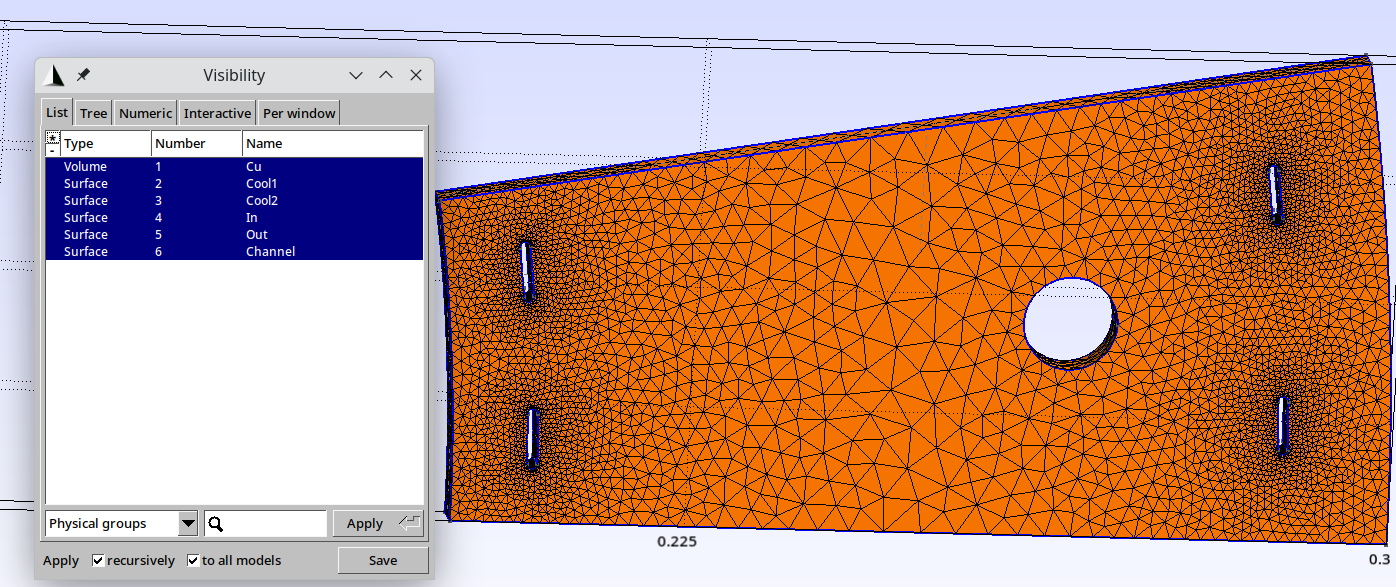
\includegraphics[width=\textwidth]{images/bitter_mesh.png}
  \caption{Adaptive 3D mesh of the LNCMI Bitter magnet.}
  \label{fig:mesh}
\end{figure}

\subsection{Mathematical model}
To model the temperature distribution in the bitter we use the well known \textbf{heat equation}:
$$
-\nabla \cdot (\kappa \nabla T) = Q \quad \text{in } \Omega,
$$
where $\kappa$ is the \textbf{thermal conductivity} of the material, $\rho$ is
the \textbf{density}, and $C_p$ is the specific \textbf{heat capacity}.

\noindent And we use the following \textbf{Poisson equation} for electric potential:
$$
- \nabla \cdot (\sigma \nabla V) = S \quad \text{in } \Omega,
$$
where $\sigma$ is the \textbf{electric conductivity} of the material.

To close the system, we use the \textbf{boundary conditions} described in
Table~\ref{tab:boundary_conditions}.

\begin{table}[H]
  \centering
  \renewcommand{\arraystretch}{1.5} % Adjust row spacing for aesthetics
  \begin{tabular}{p{3cm}p{5cm}p{4cm}}
    \toprule
    \textbf{Name} & \textbf{Heat} & \textbf{Electric} \\
    \midrule
    In & Neumann homogeneous & Dirichlet $V = 0$ \\
    Out & Neumann homogeneous & Dirichlet $V = 0.03125$ \\
    Channel & Robin ($h_e$, $T_{w,e}$) & - \\
    Cool1 & Neumann homogeneous & - \\
    Cool2 & Robin ($h_i$, $T_{w,i}$) & - \\
    \bottomrule
  \end{tabular}
  \caption{Boundary conditions.}
  \label{tab:boundary_conditions}
\end{table}

Both models are discretized using the \textbf{finite element method} (variational
formulation).

\subsection{Simulation}
\begin{minipage}[t]{0.49\textwidth}
  \justifying
  The simulations are performed on the High-Performance Computing (HPC) cluster Gaya.
  This cluster consists of a DELL PowerEdge R7525 head node and six DELL PowerEdge
  R6525 compute nodes, providing a total of 768 multi-threaded cores on the compute
  nodes and 96 cores on the head node. Gaya offers 150 TB of storage for data and
  an extremely fast 15 TB NVME scratch space. The head node is equipped with two AMD EPYC 7552 48-Core Processors running at
  2.2GHz, totaling 192 virtual cores, and 1024 GB of RAM.
  Each compute node features two AMD EPYC 7713 64-Core Processors running at 2GHz,
  totaling 256 virtual cores, and 512 GB of RAM. The nodes are interconnected via
  Broadcom Adv. Dual 10GBASE-T Ethernet and Mellanox ConnectX-6 Dx Dual Port 100
  GbE for MPI communication.
\end{minipage}
\hfill
\begin{minipage}[t]{0.49\textwidth}
  \centering
  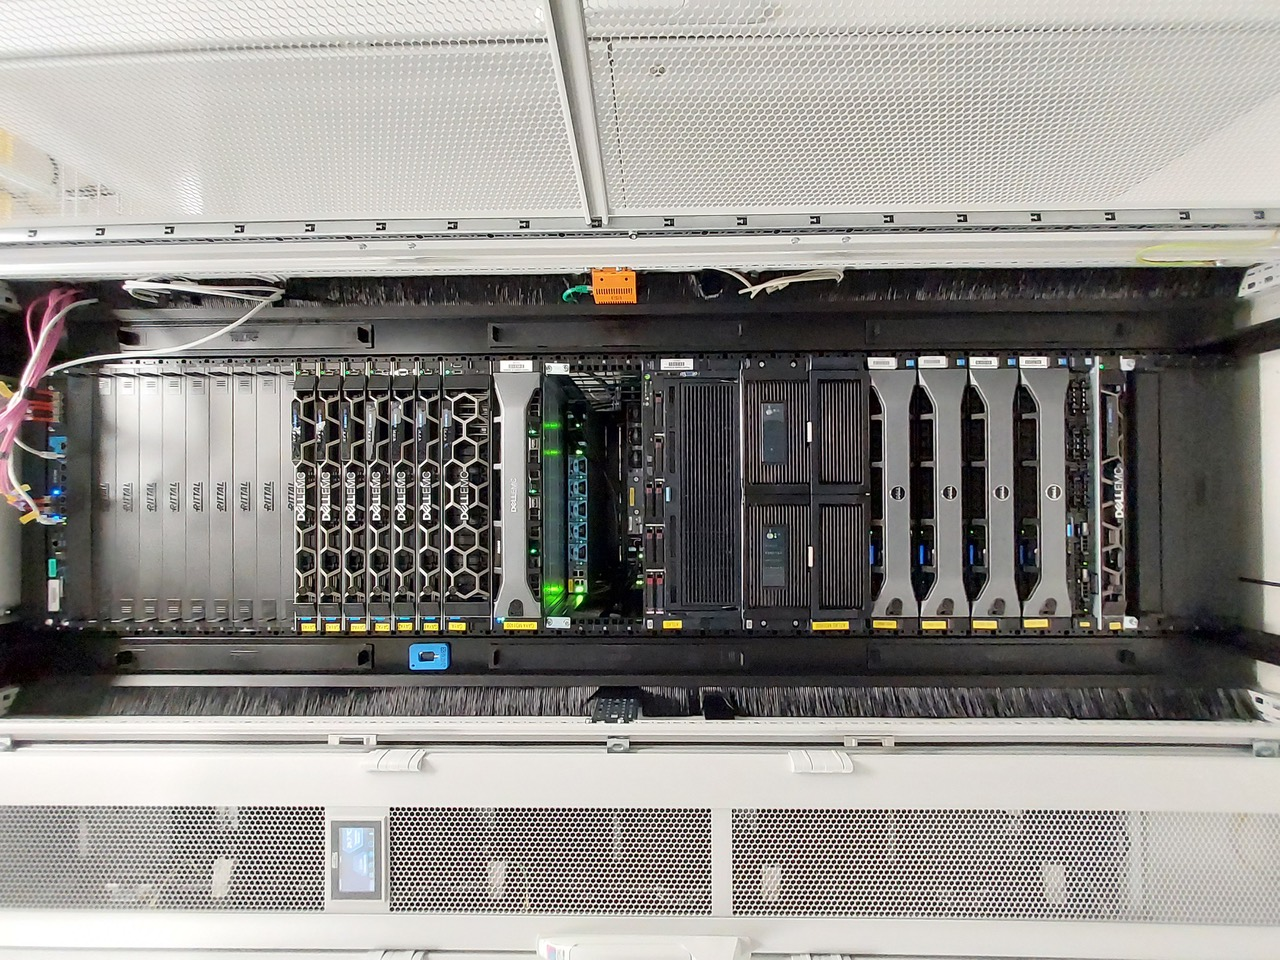
\includegraphics[width=1.1\textwidth, angle=-90]{images/gaya.jpeg}
  \captionof{figure}{Gaya supercomputer.}
\end{minipage}

We choose to use 12 processes to keep a good compromise between the parallelization
speed-up and the cost of MPI communications.

Table~\ref{tab:input_parameters} and Table~\ref{tab:physical_properties} show the
input parameters and physical properties used in the simulations.

\begin{table}[H]
  \centering
  \renewcommand{\arraystretch}{1.5} % Adjust row spacing for aesthetics
  \begin{tabular}{p{1cm}p{6cm}p{2cm}p{2cm}}
    \toprule
    \textbf{Name} & \textbf{Description} & \textbf{Value} & \textbf{Unit} \\
    \midrule
    $I$ & Current intensity & $-800$ & \SI{}{\ampere} \\
    $V_D$ & Electrical potential & $0.03125$ & \SI{}{\watt} \\
    $h_i$ & Internal transfer coefficient & $0.08$ & \SI{}{\watt mm^{-2} \kelvin^{-1}}  \\
    $T_{w,i}$ & Internal water temperature & $293$ & \SI{}{\kelvin} \\
    $h_e$ & External transfer coefficient & $0.08$ & \SI{}{\watt mm^{-2} \kelvin^{-1}} \\
    $T_{w,e}$ & External water temperature & $293$ & \SI{}{\kelvin} \\
    \bottomrule
  \end{tabular}
  \caption{Input parameters.}
  \label{tab:input_parameters}
\end{table}

\begin{table}[H]
  \centering
  \renewcommand{\arraystretch}{1.5} % Adjust row spacing for aesthetics
  \begin{tabular}{p{1cm}p{5cm}p{3cm}p{2cm}p{2cm}}
    \toprule
    \textbf{Name} & \textbf{Description} & \textbf{Marker} & \textbf{Value} & \textbf{Unit} \\
    \midrule
    $\sigma$ & Electric conductivity & omega & \SI{58e3}{} & \SI{}{\siemens mm^{-1}} \\
    $\kappa$ & Thermal conductivity & omega & $0.38$ & \SI{}{\watt mm^{-1} \kelvin^{-1}} \\
    \bottomrule
  \end{tabular}
  \caption{Physical properties (Cu).}
  \label{tab:physical_properties}
\end{table}

We perform the simulation using the Thermo-Electric toolbox of Feel++
\cite{christophe_prudhomme_feelppfeelpp_2024}, which solves the coupled system of
heat and electric potential equations in a monolithic block.
In order to be able to solve the problem on the bitter geometry
with a reasonable computational cost, we choose to use the $\mathbb{P}_1$ FEM
basis functions. The discretization parameters are summarized in Table \ref{tab:discretization}.

\begin{table}[H]
  \centering
  \begin{tabular}{@{}ll@{}}
    \toprule
    \textbf{Parameter}        & \textbf{Value}            \\ \midrule
    Dimension                 & 3                         \\
    Number of Elements       & 63,232                \\
    Number of Edges          & 86,667                \\
    Number of Faces          & 135,209                \\
    Number of Partitions     & 12                        \\
    Number of Points         & 14,686                  \\
    \( h_{\text{average}} \) & \SI{1.43e-3}{} \\
    \( h_{\text{max}} \)     & \SI{5.76e-3}{} \\
    \( h_{\text{min}} \)     & \SI{4.78e-4}{} \\
    Order                    & 1                         \\
    Real Dimension           & 3                         \\
    Shape                    & Simplex\(_{3,1,3}\)       \\ \bottomrule
  \end{tabular}
  \caption{Discretization parameters.}
  \label{tab:discretization}
\end{table}

\section{Results Visualization}
We present here some visualizations of the results obtained from the steady case simulation.
You can also visualize the results by yourself by opening the \\
\texttt{thermoelectric.exports/Export.case} file with Paraview \cite{paraview}.
Note that a \\
\texttt{thermoelectric.exports/Paraview-State.pvsm} file is also provided
to load the visualization settings.
\subsection{First views}
Figure~\ref{fig:heat_distribution} shows the heat distribution in the Bitter magnet
and Figure~\ref{fig:electric_potential} shows the electric potential distribution.
\begin{figure}[H]
  \centering
  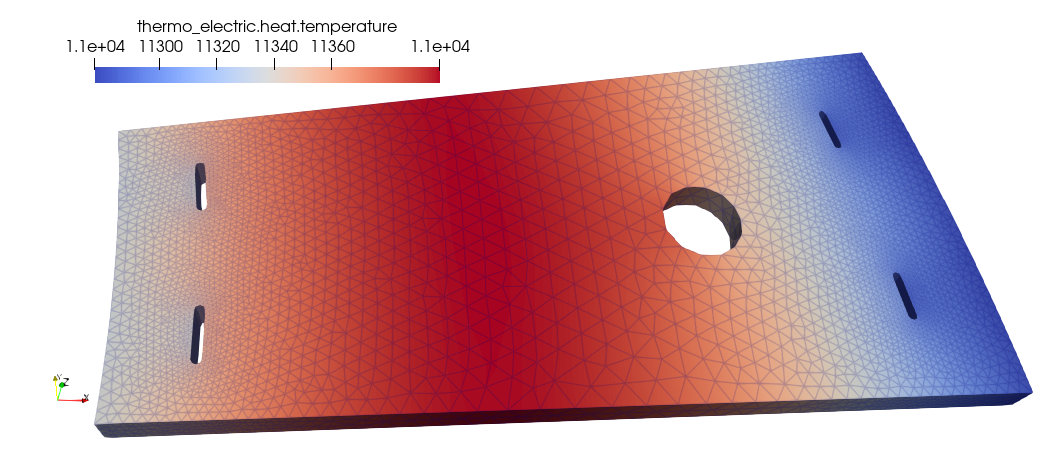
\includegraphics[width=0.8\textwidth]{images/heat.png}
  \caption{Heat distribution in the Bitter magnet [\SI{}{\kelvin}].}
  \label{fig:heat_distribution}
\end{figure}

We can see that the bigger hole (\texttt{Cool1}) is not effective to cool down the magnet, whereas
the smaller ones (\texttt{Cool2}) are better.
According to the boundary conditions settings for heat transfer (Neumann homogeneous
  for $\Gamma_{\text{cool},1}$, Robin for $\Gamma_{\text{cool},2}$ and sides
$\Gamma_{\text{channel}}$) this is a situation we were expecting to observe
in the solution.

\begin{figure}[H]
  \centering
  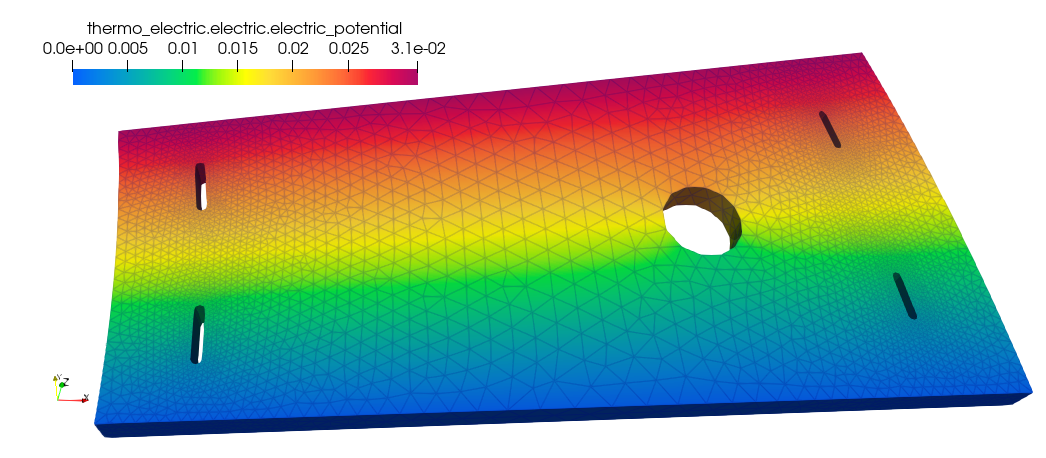
\includegraphics[width=0.8\textwidth]{images/electric_potential.png}
  \caption{Electric potential distribution in the Bitter magnet [\SI{}{\watt}].}
  \label{fig:electric_potential}
\end{figure}

As for the electric potential (Figure~\ref{fig:electric_potential}), we can see that
the potential is higher on the side of the magnet where the current inters (\texttt{In} marker)
and lower on the other side (\texttt{Out} marker). And at a first view the transition
seems to be smooth.

\subsection{Mesh topology}
Since we expect the solution to change more rapidly around the cooling holes,
we chose to use a finer mesh around them to be able to capture the solution more
precisely as shown in Figure~\ref{fig:mesh_fine}. The mesh is coarser in the
rest of the magnet as shown in Figure~\ref{fig:mesh_coarse} to reduce the computational
cost of the simulation.

\begin{figure}[H]
  \centering
  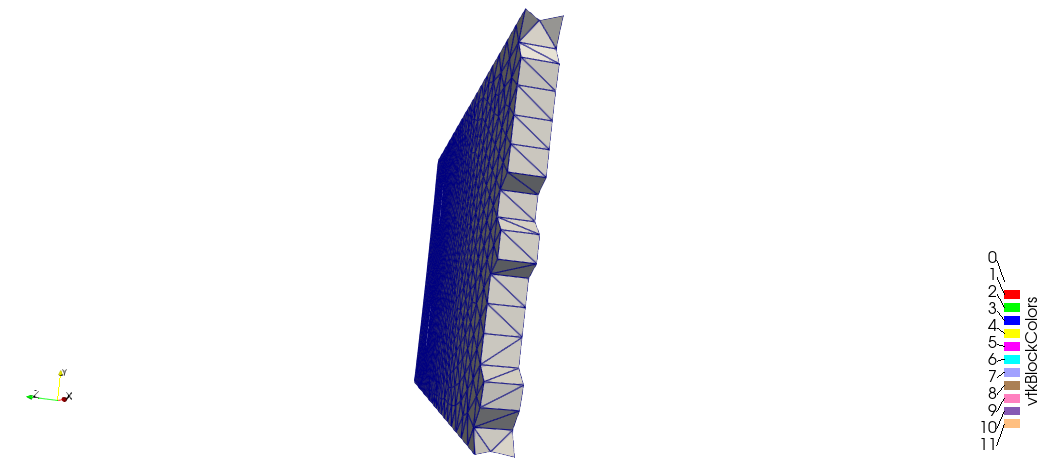
\includegraphics[width=0.8\textwidth]{images/grossier2.png}
  \caption{Cut view of the mesh at a coarse location.}
  \label{fig:mesh_coarse}
\end{figure}

\begin{figure}[H]
  \centering
  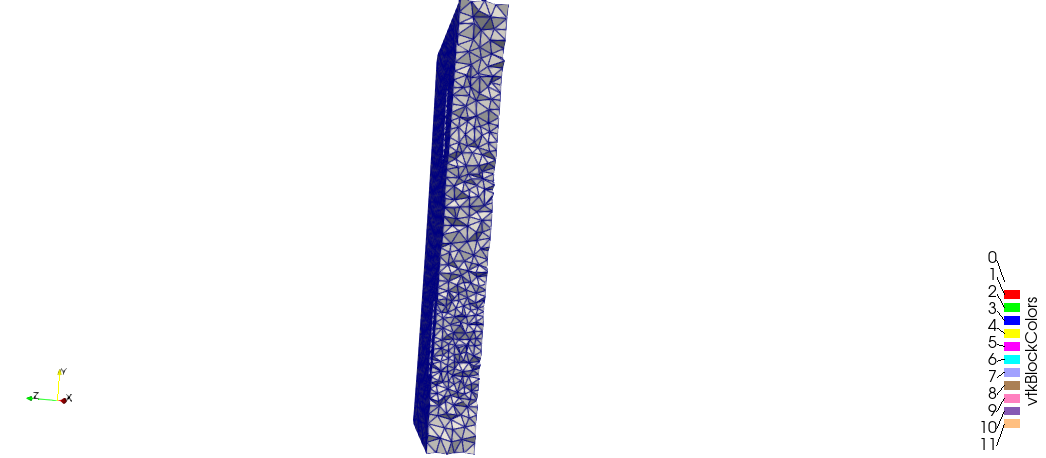
\includegraphics[width=0.8\textwidth]{images/raffiner2.png}
  \caption{Cut view of the mesh at a refined location.}
  \label{fig:mesh_fine}
\end{figure}

\subsection{Electrical field}
We can observe that the electrical field is more powerful on the inside (at the
left of the image in Figure~\ref{fig:glyph}) of the section of the magnet.
It is also the case around the holes. This is something we were expecting to
observe: indeed, as the current cannot pass through the hole, it is diverted and
thus denser around it.

\begin{figure}[H]
  \centering
  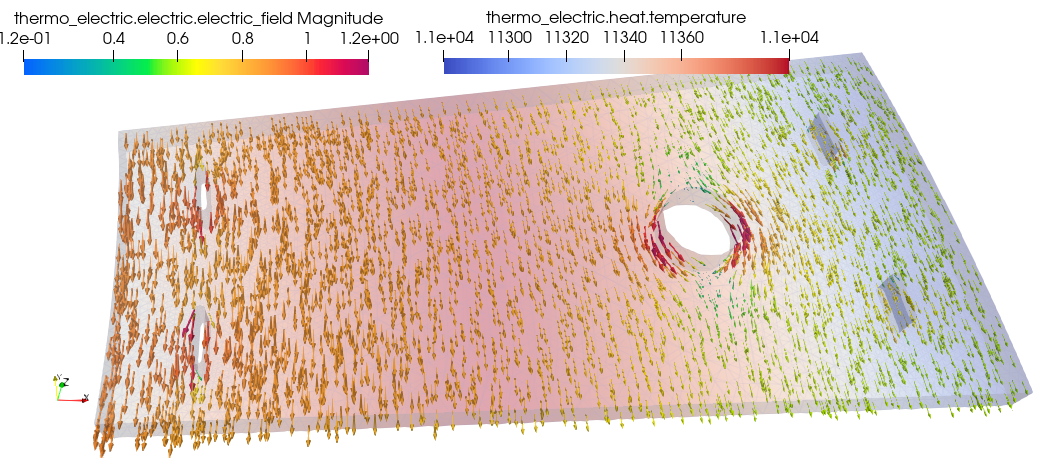
\includegraphics[width=0.8\textwidth]{images/glyph2.png}
  \caption{View of the mesh colored in function of the heat field [\SI{}{\kelvin}],
    with the vector field representing electric field orientation, colored in function
  of electric current density [\SI{}{\watt}].}
  \label{fig:glyph}
\end{figure}

\begin{figure}[H]
  \centering
  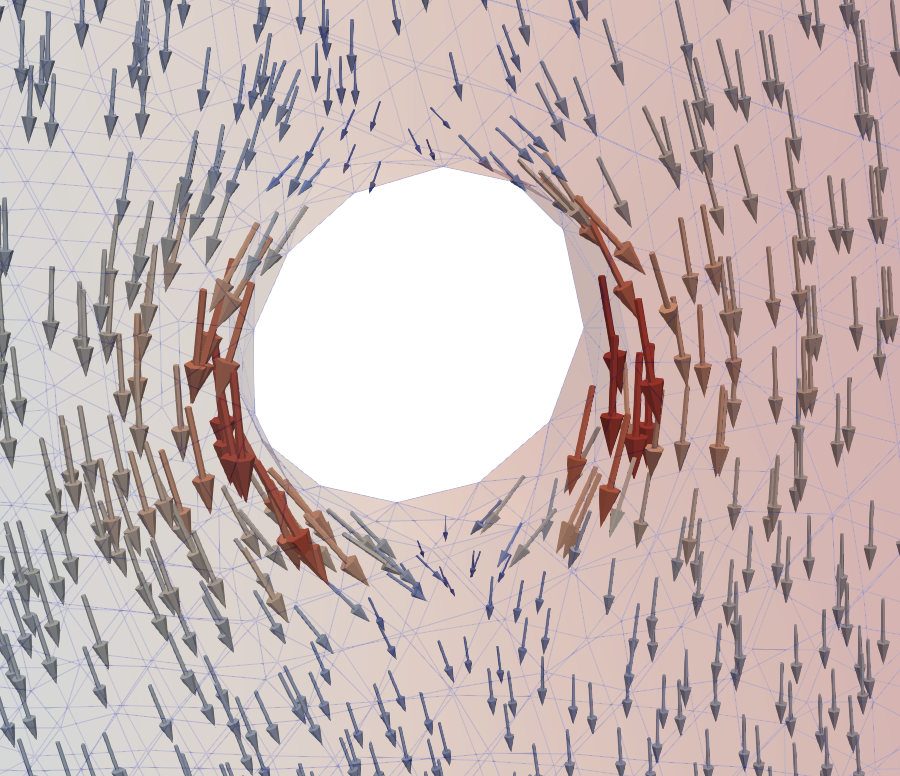
\includegraphics[width=0.8\textwidth]{images/field1_zoom.png}
  \caption{Zoom on the visualized vector field.}
  \label{fig:field1_zoom}
\end{figure}

\subsection{Surface extractions}
Figure~\ref{fig:isosurfaces} shows the extraction of the isosurfaces in the heat field,
for temperatures of 11390, 11390.5 and 11391 \SI{}{\kelvin} compared to the
electric potential distribution. The isosurfaces are distributed as follows: 11390, 11390.5, 11391 \SI{}{\kelvin} and
11390, 11390.5, 11391 \SI{}{\kelvin} again. We observe that the temperature is higher on the right
side each time, where there is more material for the current to pass through.

\begin{figure}[H]
  \centering
  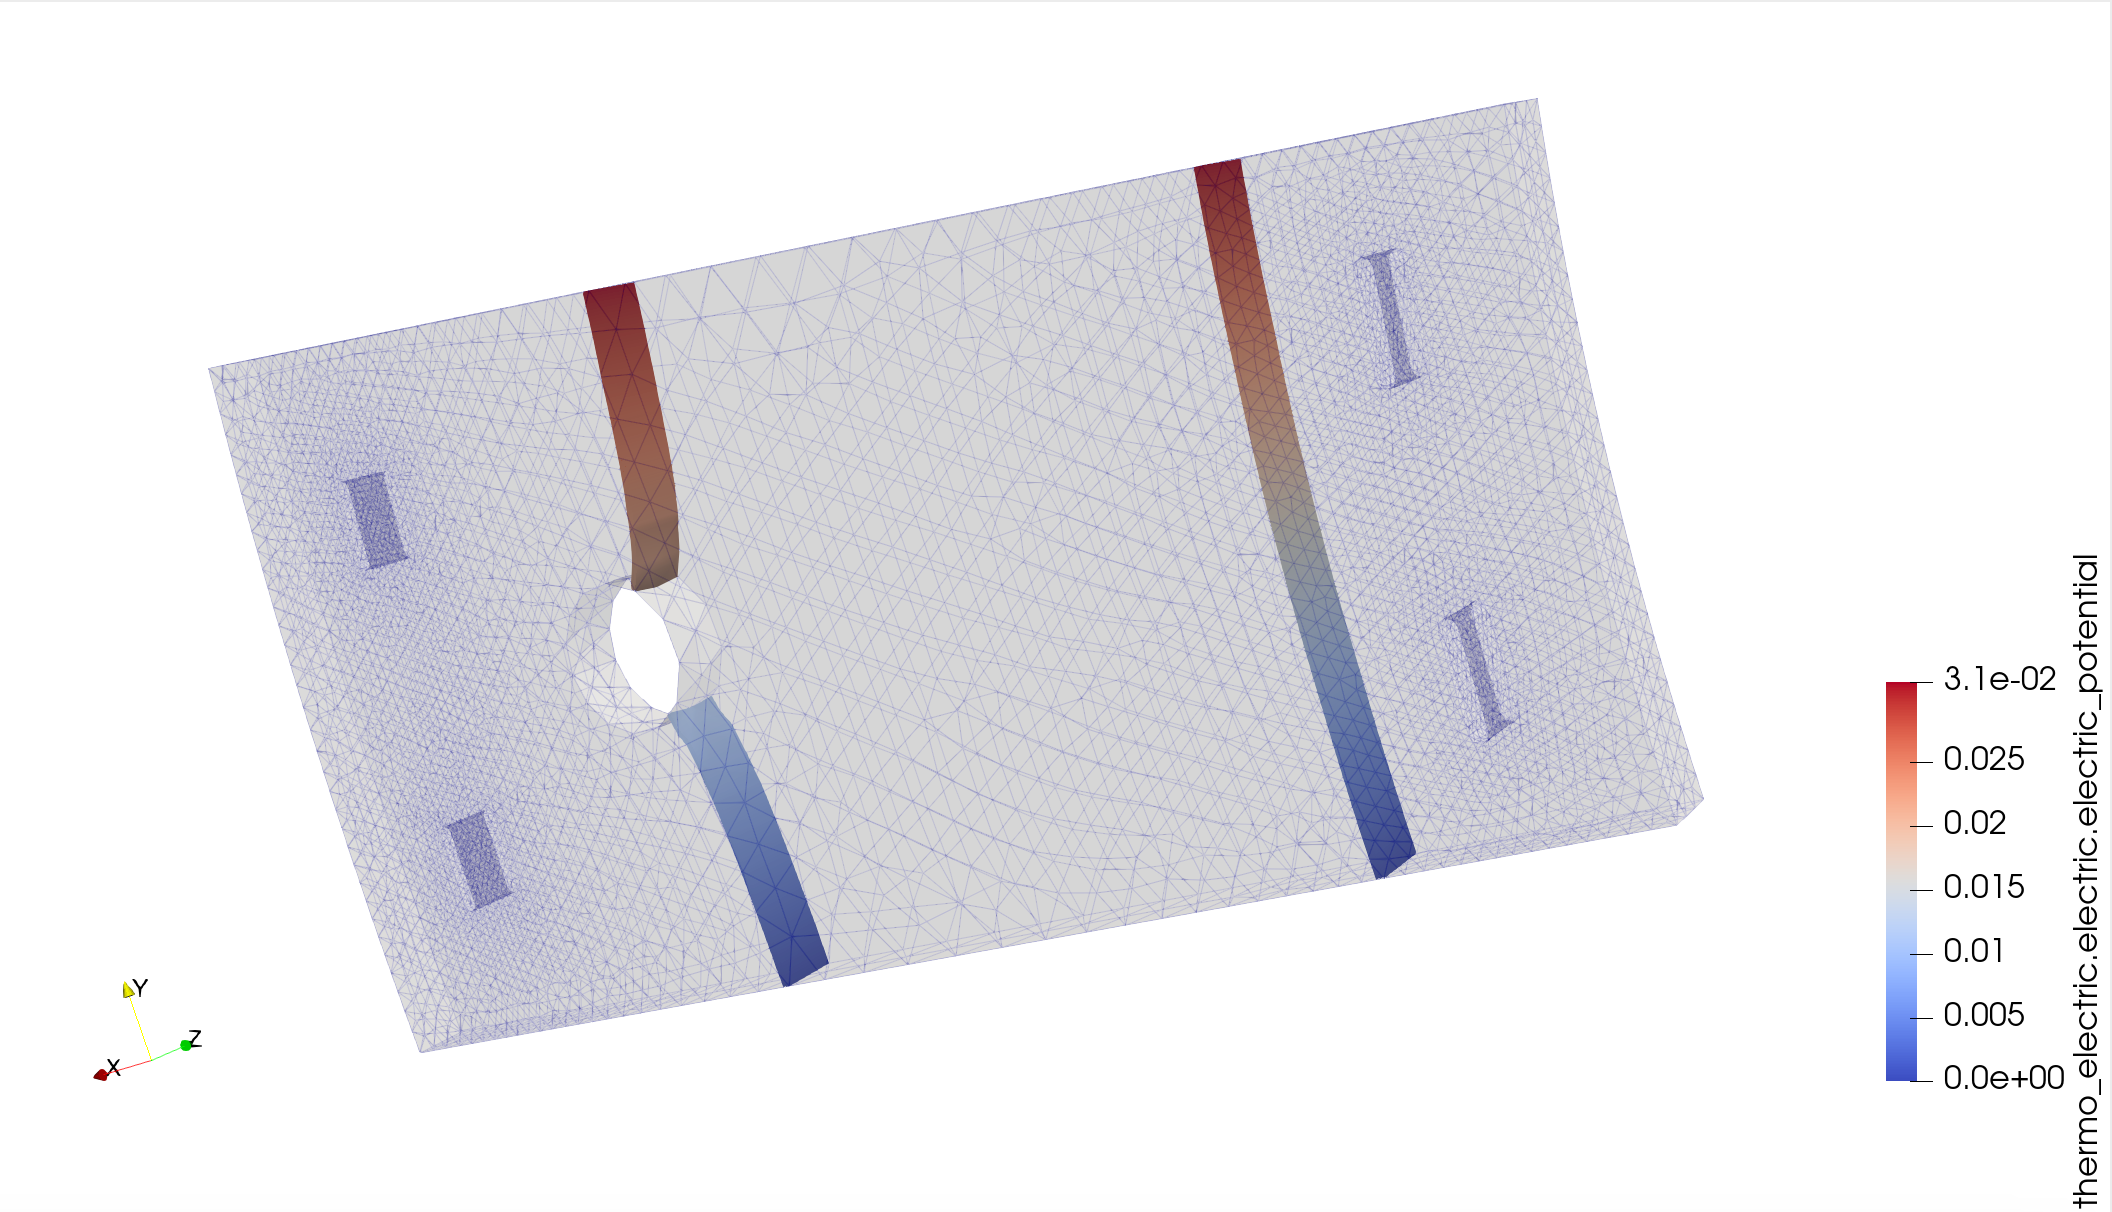
\includegraphics[width=0.8\textwidth]{images/isosurfaces.png}
  \caption{Extraction of the isosurfaces in the heat field, for temperatures of
  11390, 11390.5 and 11391 \SI{}{\kelvin}.}
  \label{fig:isosurfaces}
\end{figure}

\begin{figure}[H]
  \centering
  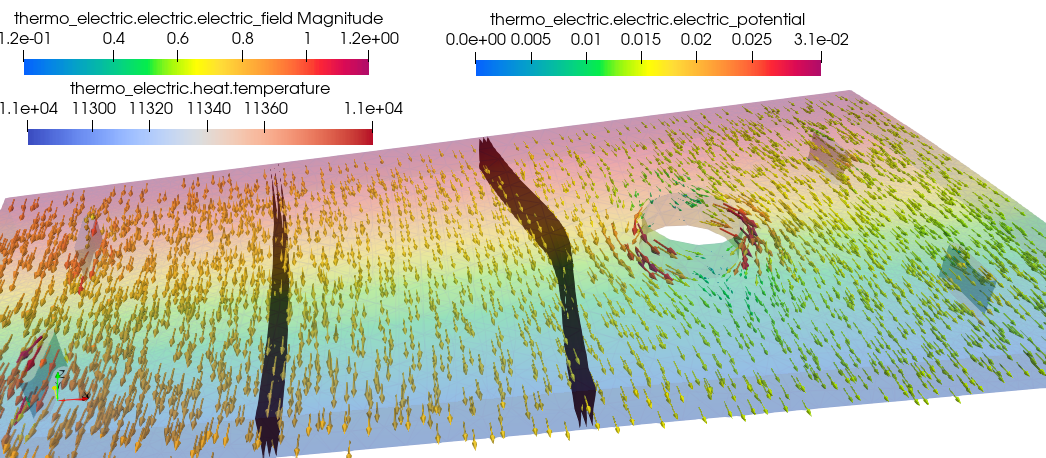
\includegraphics[width=0.8\textwidth]{images/isosurfaces_glyph.png}
  \caption{Extraction of the isosurfaces in the heat field, for temperatures of
  11390, 11390.5 and 11391 \SI{}{\kelvin} with field magnitude glyphs.}
  \label{fig:isosurfaces_glyph}
\end{figure}

We can clearly see in Figure~\ref{fig:isosurfaces_glyph} that the temperature is higher
near the hole \texttt{Cool1} where the electric field is higher, as shown in
Figure~\ref{fig:field1_zoom}.

\section{Conclusion}
In this little project, we successfully modeled and simulated the thermal and electrical
behavior of an LNCMI Bitter magnet using advanced meshing techniques and the finite
element method. By using adaptive meshing, we precisely captured critical variations
in the heat distribution and electric field within the magnet, revealing key insights
into the effectiveness of cooling mechanisms and current flow patterns. The
simulations demonstrated expected behaviors, such as localized heating and current
density around structural features like cooling holes. These results provide a
strong foundation for future optimizations, including geometry refinements, material
testing, and transient case simulations, to further enhance the magnet's performance
and reliability.

\section{Future work}
\begin{enumerate}
  \item Improve mesh slits generation by making a function to generate them.
  \item Make the mesh parametrizable to change the geometry of the Bitter magnet
    (\textit{e.g.}, radius, length, number of slits, \textit{etc.}).
  \item Test the model with different materials, physical properties, boundary conditions, \textit{etc.}
  \item Make a complexity analysis of the simulation depending on the number of elements of the mesh.
  \item Run and analyze transient cases simulations.
  \item Mesh convergence analysis.
\end{enumerate}

\newpage

\section{References}
\printbibliography
\end{document}